% ============================================================
% Question Bank: ch02-01 Solving Percent Problems (Modified — MN)
% Topic Title: Solving Percent Problems (MN percent-application emphasis)
% CCSS: 7.RP.A.3 (Modified)
% Questions: 30 (18 MC + 7 SA + 5 Graphical)
% ============================================================

% --- Multiple Choice Questions (18) ---

\begin{practiceQuestion}{m-2-1-q01}{mc}
\begin{questionText}
What is $30\%$ of $80$?
\end{questionText}
\choiceA{$2.4$}
\choiceB{$24$}
\choiceC{$240$}
\choiceD{$30$}
\correctAnswer{B}
\explanation{Convert: $30\% = 0.30$. Multiply: $0.30 \times 80 = 24$.}
\end{practiceQuestion}

\begin{practiceQuestion}{m-2-1-q02}{mc}
\begin{questionText}
A pair of shoes costs $\$75$. They are on sale for $20\%$ off. What is the sale price?
\end{questionText}
\choiceA{$\$15$}
\choiceB{$\$55$}
\choiceC{$\$60$}
\choiceD{$\$70$}
\correctAnswer{C}
\explanation{Discount: $0.20 \times 75 = \$15$. Sale price: $75 - 15 = \$60$.}
\end{practiceQuestion}

\begin{practiceQuestion}{m-2-1-q03}{mc}
\begin{questionText}
$15$ is $25\%$ of what number?
\end{questionText}
\choiceA{$3.75$}
\choiceB{$40$}
\choiceC{$60$}
\choiceD{$375$}
\correctAnswer{C}
\explanation{$15 = 0.25 \times \text{whole}$. Divide: $15 \div 0.25 = 60$.}
\end{practiceQuestion}

\begin{practiceQuestion}{m-2-1-q04}{mc}
\begin{questionText}
A meal costs $\$45$. You leave a $15\%$ tip. How much is the tip?
\end{questionText}
\choiceA{$\$4.50$}
\choiceB{$\$6.00$}
\choiceC{$\$6.75$}
\choiceD{$\$7.50$}
\correctAnswer{C}
\explanation{$0.15 \times 45 = \$6.75$.}
\end{practiceQuestion}

\begin{practiceQuestion}{m-2-1-q05}{mc}
\begin{questionText}
$18$ is what percent of $72$?
\end{questionText}
\choiceA{$4\%$}
\choiceB{$18\%$}
\choiceC{$25\%$}
\choiceD{$40\%$}
\correctAnswer{C}
\explanation{$18 \div 72 = 0.25 = 25\%$.}
\end{practiceQuestion}

\begin{practiceQuestion}{m-2-1-q06}{mc}
\begin{questionText}
A store marks up a hat from $\$14$ to $\$21$. What is the markup percent?
\end{questionText}
\choiceA{$33\%$}
\choiceB{$50\%$}
\choiceC{$67\%$}
\choiceD{$7\%$}
\correctAnswer{B}
\explanation{Markup: $21 - 14 = \$7$. Percent: $7 \div 14 = 0.50 = 50\%$.}
\end{practiceQuestion}

\begin{practiceQuestion}{m-2-1-q07}{mc}
\begin{questionText}
A tablet costs $\$200$ plus $6\%$ sales tax. What is the total cost?
\end{questionText}
\choiceA{$\$206$}
\choiceB{$\$212$}
\choiceC{$\$218$}
\choiceD{$\$260$}
\correctAnswer{B}
\explanation{Tax: $0.06 \times 200 = \$12$. Total: $200 + 12 = \$212$.}
\end{practiceQuestion}

\begin{practiceQuestion}{m-2-1-q08}{mc}
\begin{questionText}
A jacket costs $\$48$ after a $40\%$ discount. What was the original price?
\end{questionText}
\choiceA{$\$67.20$}
\choiceB{$\$80$}
\choiceC{$\$88$}
\choiceD{$\$120$}
\correctAnswer{B}
\explanation{After $40\%$ off, you pay $60\%$. $48 = 0.60 \times \text{original}$. Original: $48 \div 0.60 = \$80$.}
\end{practiceQuestion}

\begin{practiceQuestion}{m-2-1-q09}{mc}
\begin{questionText}
You spent $\$54$ on dinner including a $\$9$ tip. What percent tip did you leave on the food?
\end{questionText}
\choiceA{$\frac{1}{6} \approx 16.7\%$}
\choiceB{$20\%$}
\choiceC{$15\%$}
\choiceD{$25\%$}
\correctAnswer{B}
\explanation{Food cost: $54 - 9 = \$45$. Percent: $9 \div 45 = 0.20 = 20\%$.}
\end{practiceQuestion}

\begin{practiceQuestion}{m-2-1-q10}{mc}
\begin{questionText}
A video game costs $\$60$. It is on sale for $15\%$ off, and there is $8\%$ tax on the sale price. What do you pay?
\end{questionText}
\choiceA{$\$51.00$}
\choiceB{$\$55.08$}
\choiceC{$\$56.16$}
\choiceD{$\$58.80$}
\correctAnswer{B}
\explanation{Discount: $0.15 \times 60 = \$9$. Sale price: $60 - 9 = \$51$. Tax: $0.08 \times 51 = \$4.08$. Total: $51 + 4.08 = \$55.08$.}
\end{practiceQuestion}

\begin{practiceQuestion}{m-2-1-q11}{mc}
\begin{questionText}
A student says ``$20\%$ of $\$50$ is $\$1{,}000$'' because $20 \times 50 = 1{,}000$. What error did the student make?
\end{questionText}
\choiceA{The student forgot to convert the percent to a decimal}
\choiceB{The student should have divided, not multiplied}
\choiceC{The student used the wrong number for the whole}
\choiceD{The student's answer is actually correct}
\correctAnswer{A}
\explanation{$20\%$ must be written as $0.20$ before multiplying. $0.20 \times 50 = \$10$, not $\$1{,}000$.}
\end{practiceQuestion}

\begin{practiceQuestion}{m-2-1-q12}{mc}
\begin{questionText}
A restaurant bill is $\$32$. You want to leave a $20\%$ tip and pay $7\%$ tax on the food. What is the total amount you pay (food + tax + tip)?
\end{questionText}
\choiceA{$\$40.64$}
\choiceB{$\$41.24$}
\choiceC{$\$40.24$}
\choiceD{$\$42.64$}
\correctAnswer{A}
\explanation{Tax: $0.07 \times 32 = \$2.24$. Tip: $0.20 \times 32 = \$6.40$. Total: $32 + 2.24 + 6.40 = \$40.64$.}
\end{practiceQuestion}

\begin{practiceQuestion}{m-2-1-q13}{mc}
\begin{questionText}
A store buys a sweater for $\$25$ and sells it for $\$40$. What is the markup percent?
\end{questionText}
\choiceA{$37.5\%$}
\choiceB{$60\%$}
\choiceC{$62.5\%$}
\choiceD{$15\%$}
\correctAnswer{B}
\explanation{Markup: $40 - 25 = \$15$. Percent: $15 \div 25 = 0.60 = 60\%$.}
\end{practiceQuestion}

\begin{practiceQuestion}{m-2-1-q14}{mc}
\begin{questionText}
A phone originally costs $\$350$. It is discounted $30\%$. Then an additional $10\%$ is taken off the sale price. What is the final price?
\end{questionText}
\choiceA{$\$210.00$}
\choiceB{$\$220.50$}
\choiceC{$\$245.00$}
\choiceD{$\$140.00$}
\correctAnswer{B}
\explanation{First discount: $0.30 \times 350 = \$105$. Sale price: $350 - 105 = \$245$. Second discount: $0.10 \times 245 = \$24.50$. Final: $245 - 24.50 = \$220.50$.}
\end{practiceQuestion}

\begin{practiceQuestion}{m-2-1-q15}{mc}
\begin{questionText}
Which expression gives $8\%$ sales tax on a $\$65$ item?
\end{questionText}
\choiceA{$65 \times 8$}
\choiceB{$65 \times 0.8$}
\choiceC{$65 \times 0.08$}
\choiceD{$65 \div 0.08$}
\correctAnswer{C}
\explanation{$8\% = 0.08$. Tax $= 65 \times 0.08 = \$5.20$.}
\end{practiceQuestion}

\begin{practiceQuestion}{m-2-1-q16}{mc}
\begin{questionText}
A bike is on sale for $\$180$ after a $25\%$ discount. A student says the original price was $\$225$. Is the student correct?
\end{questionText}
\choiceA{No — the original price was $\$240$}
\choiceB{No — the original price was $\$205$}
\choiceC{Yes — $\$225$ is correct}
\choiceD{No — the original price was $\$144$}
\correctAnswer{A}
\explanation{After $25\%$ off, you pay $75\%$. $180 = 0.75 \times \text{original}$. Original: $180 \div 0.75 = \$240$, not $\$225$.}
\end{practiceQuestion}

\begin{practiceQuestion}{m-2-1-q17}{mc}
\begin{questionText}
A coupon gives $\$10$ off an item that costs $\$80$. What percent discount is the coupon?
\end{questionText}
\choiceA{$8\%$}
\choiceB{$10\%$}
\choiceC{$12.5\%$}
\choiceD{$15\%$}
\correctAnswer{C}
\explanation{$10 \div 80 = 0.125 = 12.5\%$.}
\end{practiceQuestion}

\begin{practiceQuestion}{m-2-1-q18}{mc}
\begin{questionText}
A waiter earns $\$56$ in tips on $\$280$ worth of food orders. What percent tip did the customers leave on average?
\end{questionText}
\choiceA{$15\%$}
\choiceB{$18\%$}
\choiceC{$20\%$}
\choiceD{$25\%$}
\correctAnswer{C}
\explanation{$56 \div 280 = 0.20 = 20\%$.}
\end{practiceQuestion}

% --- Short Answer Questions (7) ---

\begin{practiceQuestion}{m-2-1-q19}{sa}
\begin{questionText}
What is $45\%$ of $120$?
\end{questionText}
\correctAnswer{$54$}
\explanation{$0.45 \times 120 = 54$.}
\end{practiceQuestion}

\begin{practiceQuestion}{m-2-1-q20}{sa}
\begin{questionText}
A shirt costs $\$28$ before tax. With $7.5\%$ sales tax, what is the total cost?
\end{questionText}
\correctAnswer{$\$30.10$}
\explanation{Tax: $0.075 \times 28 = \$2.10$. Total: $28 + 2.10 = \$30.10$.}
\end{practiceQuestion}

\begin{practiceQuestion}{m-2-1-q21}{sa}
\begin{questionText}
A store sells a book for $\$24$. The store's cost was $\$16$. What is the markup percent?
\end{questionText}
\correctAnswer{$50\%$}
\explanation{Markup: $24 - 16 = \$8$. Percent: $8 \div 16 = 0.50 = 50\%$.}
\end{practiceQuestion}

\begin{practiceQuestion}{m-2-1-q22}{sa}
\begin{questionText}
A bicycle costs $\$160$ after a $20\%$ discount. What was the original price?
\end{questionText}
\correctAnswer{$\$200$}
\explanation{You pay $80\%$: $160 = 0.80 \times \text{original}$. Original: $160 \div 0.80 = \$200$.}
\end{practiceQuestion}

\begin{practiceQuestion}{m-2-1-q23}{sa}
\begin{questionText}
A family's dinner bill is $\$65$. They leave a $\$13$ tip. What percent tip is this?
\end{questionText}
\correctAnswer{$20\%$}
\explanation{$13 \div 65 = 0.20 = 20\%$.}
\end{practiceQuestion}

\begin{practiceQuestion}{m-2-1-q24}{sa}
\begin{questionText}
$36$ is what percent of $90$?
\end{questionText}
\correctAnswer{$40\%$}
\explanation{$36 \div 90 = 0.40 = 40\%$.}
\end{practiceQuestion}

\begin{practiceQuestion}{m-2-1-q25}{sa}
\begin{questionText}
A skateboard costs $\$55$ plus $9\%$ tax. You have $\$60$. Do you have enough money? Explain.
\end{questionText}
\correctAnswer{$\$59.95$; yes, barely enough}
\explanation{Tax: $0.09 \times 55 = \$4.95$. Total: $55 + 4.95 = \$59.95$. Since $\$59.95 < \$60$, you have just enough.}
\end{practiceQuestion}

% --- Graphical Questions (3 GMC + 2 GSA) ---

\begin{practiceQuestion}{m-2-1-q26}{gmc}
\begin{questionText}
The bar model below represents the original price of a jacket. The shaded part shows the discount. What is the sale price?

\begin{center}
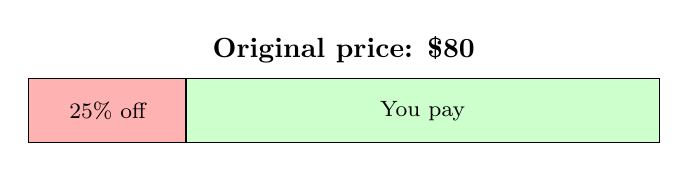
\begin{tikzpicture}[scale=0.8]
  \draw[thick] (0,0) rectangle (10,1);
  \fill[red!30] (0,0) rectangle (2.5,1);
  \fill[green!20] (2.5,0) rectangle (10,1);
  \draw[thick] (2.5,0) -- (2.5,1);
  \node at (1.25,0.5) {\footnotesize $25\%$ off};
  \node at (6.25,0.5) {\footnotesize You pay};
  \node[above] at (5,1.1) {\textbf{Original price: \$80}};
\end{tikzpicture}
\end{center}
\end{questionText}
\choiceA{$\$20$}
\choiceB{$\$55$}
\choiceC{$\$60$}
\choiceD{$\$75$}
\correctAnswer{C}
\explanation{$25\%$ of $\$80 = \$20$ discount. Sale price: $80 - 20 = \$60$.}
\end{practiceQuestion}

\begin{practiceQuestion}{m-2-1-q27}{gmc}
\begin{questionText}
The circle graph shows how a student spent $\$200$.

\begin{center}
\begin{tikzpicture}[scale=1.2]
  \fill[funBlue!40] (0,0) -- (0,1.5) arc(90:90-0.4*360:1.5) -- cycle;
  \fill[funGreen!40] (0,0) -- (90-0.4*360:1.5) arc(90-0.4*360:90-0.65*360:1.5) -- cycle;
  \fill[funOrange!40] (0,0) -- (90-0.65*360:1.5) arc(90-0.65*360:90-0.85*360:1.5) -- cycle;
  \fill[red!30] (0,0) -- (90-0.85*360:1.5) arc(90-0.85*360:90-1.0*360:1.5) -- cycle;
  \draw[thick] (0,0) circle(1.5);
  \node at (90-0.2*360:1) {\footnotesize $40\%$};
  \node at (90-0.525*360:1) {\footnotesize $25\%$};
  \node at (90-0.75*360:1) {\footnotesize $20\%$};
  \node at (90-0.925*360:1) {\footnotesize $15\%$};
  \node[right] at (1.8,1) {\footnotesize Clothes};
  \node[right] at (1.8,0.4) {\footnotesize Food};
  \node[right] at (1.8,-0.2) {\footnotesize Books};
  \node[right] at (1.8,-0.8) {\footnotesize Savings};
\end{tikzpicture}
\end{center}

How much did the student spend on food?
\end{questionText}
\choiceA{$\$25$}
\choiceB{$\$40$}
\choiceC{$\$50$}
\choiceD{$\$80$}
\correctAnswer{C}
\explanation{Food is $25\%$ of $\$200$. $0.25 \times 200 = \$50$.}
\end{practiceQuestion}

\begin{practiceQuestion}{m-2-1-q28}{gmc}
\begin{questionText}
The table shows prices before and after a markup. Which item has the greatest markup percent?

\begin{center}
\begin{tabular}{|l|c|c|}
\hline
\textbf{Item} & \textbf{Cost} & \textbf{Selling Price} \\
\hline
Hat & $\$10$ & $\$16$ \\
\hline
Scarf & $\$8$ & $\$12$ \\
\hline
Gloves & $\$15$ & $\$21$ \\
\hline
\end{tabular}
\end{center}
\end{questionText}
\choiceA{Hat}
\choiceB{Scarf}
\choiceC{Gloves}
\choiceD{They are all the same}
\correctAnswer{A}
\explanation{Hat: $(16-10)/10 = 60\%$. Scarf: $(12-8)/8 = 50\%$. Gloves: $(21-15)/15 = 40\%$. Hat has the highest markup.}
\end{practiceQuestion}

\begin{practiceQuestion}{m-2-1-q29}{gsa}
\begin{questionText}
The $10 \times 10$ grid represents a whole. What percent of the grid is shaded, and what number does the shaded part represent if the whole is $\$150$?

\begin{center}
\begin{tikzpicture}[scale=0.35]
  \foreach \x in {0,...,9} {
    \foreach \y in {0,...,9} {
      \draw (\x,\y) rectangle (\x+1,\y+1);
    }
  }
  % Shade 35 squares (rows 0–2 fully = 30, row 3 first 5 = 35)
  \foreach \x in {0,...,9} {
    \foreach \y in {0,...,2} {
      \fill[funBlue!40] (\x,\y) rectangle (\x+1,\y+1);
    }
  }
  \foreach \x in {0,...,4} {
    \fill[funBlue!40] (\x,3) rectangle (\x+1,4);
  }
\end{tikzpicture}
\end{center}
\end{questionText}
\correctAnswer{$35\%$; $\$52.50$}
\explanation{$35$ out of $100$ squares are shaded $= 35\%$. $0.35 \times 150 = \$52.50$.}
\end{practiceQuestion}

\begin{practiceQuestion}{m-2-1-q30}{gsa}
\begin{questionText}
Use the receipt below. Find the tax amount and the total.

\begin{center}
\begin{tabular}{|l r|}
\hline
\multicolumn{2}{|c|}{\textbf{Store Receipt}} \\
\hline
Jeans & $\$35.00$ \\
T-shirt & $\$15.00$ \\
\hline
Subtotal & $\$50.00$ \\
Tax ($6\%$) & ? \\
\hline
\textbf{Total} & \textbf{?} \\
\hline
\end{tabular}
\end{center}
\end{questionText}
\correctAnswer{Tax $= \$3.00$; Total $= \$53.00$}
\explanation{Tax: $0.06 \times 50 = \$3.00$. Total: $50 + 3 = \$53.00$.}
\end{practiceQuestion}
